\documentclass{standalone}
\usepackage{tikz}
\usetikzlibrary{patterns}
\usetikzlibrary{positioning}
\usetikzlibrary{patterns, positioning}
\usetikzlibrary{shapes.misc}
\usepackage[outline]{contour}
\contourlength{1.5pt} 
\usetikzlibrary{calc}
        \usepackage{relsize}
        \tikzset{fontscale/.style = {font=\relsize{#1}}}

\begin{document}
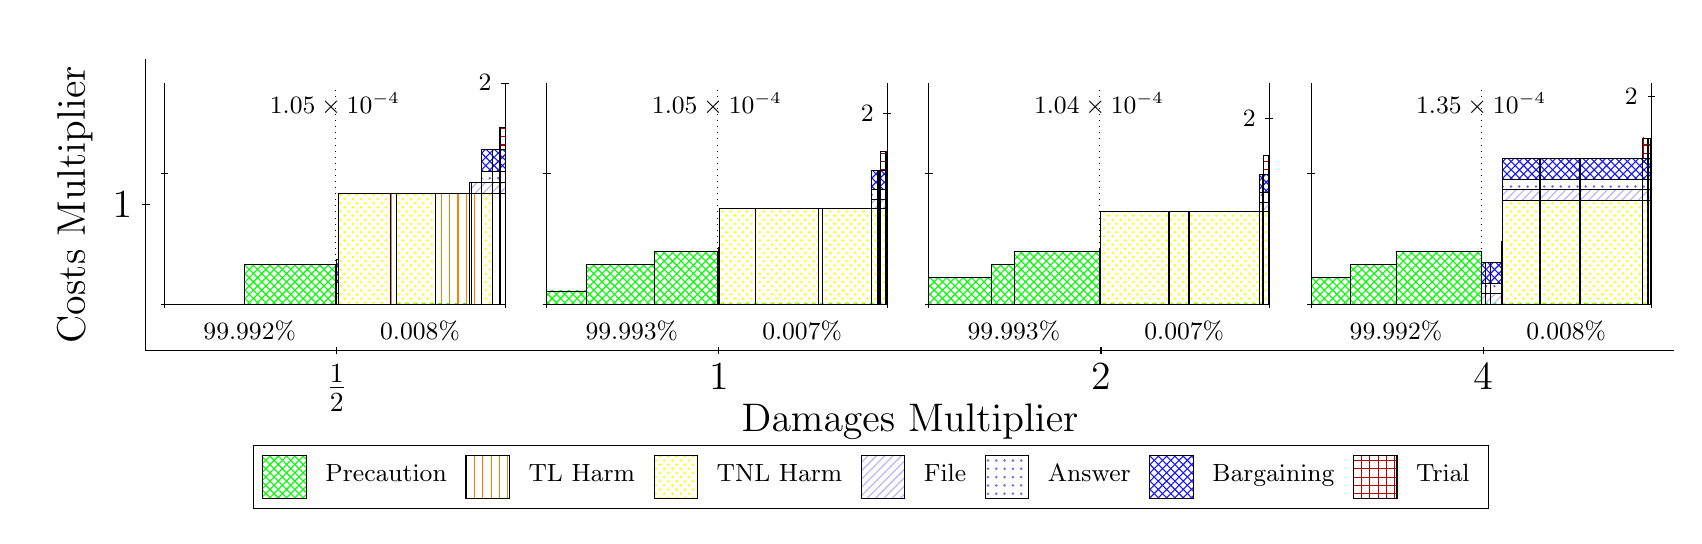
\begin{tikzpicture}
\clip(-0.5,-1.1) rectangle +(20.91,6.2);
\draw[black] (1,1) -- (1,4.7);
\node[rotate=90, fontscale=2, anchor=center] at (0.1, 2.85) {Costs Multiplier};
\draw[black] (0.95,2.85) -- (1.05,2.85);
\node[fontscale=2, anchor=east] at (0.95, 2.85) {1};

\draw[black] (1,1) -- (20.41,1);
\node[fontscale=2, anchor=center] at (10.705, 0.1) {Damages Multiplier};
\draw[black] (3.4263,0.95) -- (3.4263,1.05);
\node[fontscale=2, anchor=north] at (3.4263, 0.95) {$\frac{1}{2}$};
\draw[black] (8.2788,0.95) -- (8.2788,1.05);
\node[fontscale=2, anchor=north] at (8.2788, 0.95) {1};
\draw[black] (13.131,0.95) -- (13.131,1.05);
\node[fontscale=2, anchor=north] at (13.131, 0.95) {2};
\draw[black] (17.984,0.95) -- (17.984,1.05);
\node[fontscale=2, anchor=north] at (17.984, 0.95) {4};


\draw[pattern=crosshatch, pattern color=green,draw=black,very thin] (2.25,1.592) rectangle (3.4013,2.09);
\draw[pattern=north east lines, pattern color=blue!30,draw=black,very thin] (3.4013,1.592) rectangle (3.4168,1.7324);
\draw[pattern=north east lines, pattern color=blue!30,draw=black,very thin] (3.4168,1.592) rectangle (3.4395,1.7324);
\draw[pattern=dots,  pattern color=blue!60,draw=black,very thin] (3.4168,1.7324) rectangle (3.4395,1.8728);
\draw[pattern=crosshatch,      pattern color=blue!90,draw=black,very thin] (3.4168,1.8728) rectangle (3.4395,2.1536);
\draw[pattern=north east lines, pattern color=blue!30,draw=black,very thin] (3.4395,1.592) rectangle (3.4471,1.7324);
\draw[pattern=dots,  pattern color=blue!60,draw=black,very thin] (3.4395,1.7324) rectangle (3.4471,1.8728);
\draw[pattern=crosshatch,      pattern color=blue!90,draw=black,very thin] (3.4395,1.8728) rectangle (3.4471,2.1536);
\draw[pattern=grid,            pattern color=red!70!black,draw=black,very thin] (3.4395,2.1536) rectangle (3.4471,2.4344);
\draw[pattern=crosshatch dots, pattern color=yellow,draw=black,very thin] (3.4471,1.592) rectangle (4.1055,2.996);
\draw[pattern=vertical lines, pattern color=orange,draw=black,very thin] (4.1055,1.592) rectangle (4.1849,2.996);
\draw[pattern=crosshatch, pattern color=green,draw=black,very thin] (4.1849,1.592) rectangle (4.6815,1.592);
\draw[pattern=crosshatch dots, pattern color=yellow,draw=black,very thin] (4.1849,1.592) rectangle (4.6815,2.996);
\draw[pattern=crosshatch, pattern color=green,draw=black,very thin] (4.6815,1.592) rectangle (5.1057,1.592);
\draw[pattern=vertical lines, pattern color=orange,draw=black,very thin] (4.6815,1.592) rectangle (5.1057,2.996);
\draw[pattern=crosshatch dots, pattern color=yellow,draw=black,very thin] (5.1057,1.592) rectangle (5.1349,2.996);
\draw[pattern=north east lines, pattern color=blue!30,draw=black,very thin] (5.1057,2.996) rectangle (5.1349,3.1364);
\draw[pattern=vertical lines, pattern color=orange,draw=black,very thin] (5.1349,1.592) rectangle (5.2609,2.996);
\draw[pattern=north east lines, pattern color=blue!30,draw=black,very thin] (5.1349,2.996) rectangle (5.2609,3.1364);
\draw[pattern=crosshatch dots, pattern color=yellow,draw=black,very thin] (5.2609,1.592) rectangle (5.4037,2.996);
\draw[pattern=north east lines, pattern color=blue!30,draw=black,very thin] (5.2609,2.996) rectangle (5.4037,3.1364);
\draw[pattern=dots,  pattern color=blue!60,draw=black,very thin] (5.2609,3.1364) rectangle (5.4037,3.2768);
\draw[pattern=crosshatch,      pattern color=blue!90,draw=black,very thin] (5.2609,3.2768) rectangle (5.4037,3.5576);
\draw[pattern=vertical lines, pattern color=orange,draw=black,very thin] (5.4037,1.592) rectangle (5.4882,2.996);
\draw[pattern=north east lines, pattern color=blue!30,draw=black,very thin] (5.4037,2.996) rectangle (5.4882,3.1364);
\draw[pattern=dots,  pattern color=blue!60,draw=black,very thin] (5.4037,3.1364) rectangle (5.4882,3.2768);
\draw[pattern=crosshatch,      pattern color=blue!90,draw=black,very thin] (5.4037,3.2768) rectangle (5.4882,3.5576);
\draw[pattern=crosshatch dots, pattern color=yellow,draw=black,very thin] (5.4882,1.592) rectangle (5.5053,2.996);
\draw[pattern=north east lines, pattern color=blue!30,draw=black,very thin] (5.4882,2.996) rectangle (5.5053,3.1364);
\draw[pattern=dots,  pattern color=blue!60,draw=black,very thin] (5.4882,3.1364) rectangle (5.5053,3.2768);
\draw[pattern=crosshatch,      pattern color=blue!90,draw=black,very thin] (5.4882,3.2768) rectangle (5.5053,3.5576);
\draw[pattern=grid,            pattern color=red!70!black,draw=black,very thin] (5.4882,3.5576) rectangle (5.5053,3.8384);
\draw[pattern=vertical lines, pattern color=orange,draw=black,very thin] (5.5053,1.592) rectangle (5.5644,2.996);
\draw[pattern=north east lines, pattern color=blue!30,draw=black,very thin] (5.5053,2.996) rectangle (5.5644,3.1364);
\draw[pattern=dots,  pattern color=blue!60,draw=black,very thin] (5.5053,3.1364) rectangle (5.5644,3.2768);
\draw[pattern=crosshatch,      pattern color=blue!90,draw=black,very thin] (5.5053,3.2768) rectangle (5.5644,3.5576);
\draw[pattern=grid,            pattern color=red!70!black,draw=black,very thin] (5.5053,3.5576) rectangle (5.5644,3.8384);
\node[font=\small,text=black,anchor=north] at (3.4013, 4.4) {$1.05\times 10^{-4}$};
\draw[black,very thin] (1.2381,1.592) -- (1.2381,4.4);
\draw[black,very thin] (1.1881,1.592) -- (1.2881,1.592);
\node[font=\small,text=black, anchor=west] at (1.1881, 1.592) {};
\draw[black,very thin] (1.1881,3.2519) -- (1.2881,3.2519);
\node[font=\small,text=black, anchor=west] at (1.1881, 3.2519) {};

\draw[black,dotted,very thin] (3.4013,1.6762) -- (3.4013,4.3158);
\draw[black,very thin] (5.5644,1.592) -- (5.5644,4.4);
\draw[black,very thin] (5.5144,4.4) -- (5.6144,4.4);
\node[font=\small,text=black, anchor=east] at (5.5144, 4.4) {\contour{white}{2}};

\draw[black,very thin] (1.2381,1.592) -- (5.5644,1.592);
\draw[black,very thin] (1.2381,1.542) -- (1.2381,1.642);
\node[font=\small,text=black, anchor=north] at (1.2381, 1.542) {};
\draw[black,very thin] (5.5644,1.542) -- (5.5644,1.642);
\node[font=\small,text=black, anchor=north] at (5.5644, 1.542) {};

\node[font=\small,text=black,anchor=south] at (2.3197, 0.992) {99.992\%};
\node[font=\small,text=black,anchor=south] at (4.4828, 0.992) {0.008\%};

\draw[pattern=crosshatch, pattern color=green,draw=black,very thin] (6.0906,1.592) rectangle (6.5882,1.758);
\draw[pattern=crosshatch, pattern color=green,draw=black,very thin] (6.5882,1.592) rectangle (7.4639,2.09);
\draw[pattern=crosshatch, pattern color=green,draw=black,very thin] (7.4639,1.592) rectangle (8.2538,2.256);
\draw[pattern=crosshatch, pattern color=green,draw=black,very thin] (8.2538,1.592) rectangle (8.2642,1.592);
\draw[pattern=north east lines, pattern color=blue!30,draw=black,very thin] (8.2538,1.592) rectangle (8.2642,1.7128);
\draw[pattern=dots,  pattern color=blue!60,draw=black,very thin] (8.2538,1.7128) rectangle (8.2642,1.8337);
\draw[pattern=crosshatch,      pattern color=blue!90,draw=black,very thin] (8.2538,1.8337) rectangle (8.2642,2.0753);
\draw[pattern=crosshatch, pattern color=green,draw=black,very thin] (8.2642,1.592) rectangle (8.2681,1.592);
\draw[pattern=north east lines, pattern color=blue!30,draw=black,very thin] (8.2642,1.592) rectangle (8.2681,1.7129);
\draw[pattern=dots,  pattern color=blue!60,draw=black,very thin] (8.2642,1.7129) rectangle (8.2681,1.8337);
\draw[pattern=crosshatch,      pattern color=blue!90,draw=black,very thin] (8.2642,1.8337) rectangle (8.2681,2.0753);
\draw[pattern=crosshatch, pattern color=green,draw=black,very thin] (8.2681,1.592) rectangle (8.2757,1.592);
\draw[pattern=north east lines, pattern color=blue!30,draw=black,very thin] (8.2681,1.592) rectangle (8.2757,1.7128);
\draw[pattern=dots,  pattern color=blue!60,draw=black,very thin] (8.2681,1.7128) rectangle (8.2757,1.8337);
\draw[pattern=crosshatch,      pattern color=blue!90,draw=black,very thin] (8.2681,1.8337) rectangle (8.2757,2.0753);
\draw[pattern=grid,            pattern color=red!70!black,draw=black,very thin] (8.2681,2.0753) rectangle (8.2757,2.317);
\draw[pattern=crosshatch, pattern color=green,draw=black,very thin] (8.2757,1.592) rectangle (8.2782,1.592);
\draw[pattern=north east lines, pattern color=blue!30,draw=black,very thin] (8.2757,1.592) rectangle (8.2782,1.7129);
\draw[pattern=dots,  pattern color=blue!60,draw=black,very thin] (8.2757,1.7129) rectangle (8.2782,1.8337);
\draw[pattern=crosshatch,      pattern color=blue!90,draw=black,very thin] (8.2757,1.8337) rectangle (8.2782,2.0753);
\draw[pattern=grid,            pattern color=red!70!black,draw=black,very thin] (8.2757,2.0753) rectangle (8.2782,2.317);
\draw[pattern=crosshatch, pattern color=green,draw=black,very thin] (8.2782,1.592) rectangle (8.7427,1.592);
\draw[pattern=crosshatch dots, pattern color=yellow,draw=black,very thin] (8.2782,1.592) rectangle (8.7427,2.8003);
\draw[pattern=crosshatch, pattern color=green,draw=black,very thin] (8.7427,1.592) rectangle (8.7454,1.592);
\draw[pattern=vertical lines, pattern color=orange,draw=black,very thin] (8.7427,1.592) rectangle (8.7454,2.8003);
\draw[pattern=crosshatch, pattern color=green,draw=black,very thin] (8.7454,1.592) rectangle (9.5343,1.592);
\draw[pattern=crosshatch dots, pattern color=yellow,draw=black,very thin] (8.7454,1.592) rectangle (9.5343,2.8003);
\draw[pattern=crosshatch, pattern color=green,draw=black,very thin] (9.5343,1.592) rectangle (9.5912,1.592);
\draw[pattern=vertical lines, pattern color=orange,draw=black,very thin] (9.5343,1.592) rectangle (9.5912,2.8003);
\draw[pattern=crosshatch, pattern color=green,draw=black,very thin] (9.5912,1.592) rectangle (10.21,1.592);
\draw[pattern=crosshatch dots, pattern color=yellow,draw=black,very thin] (9.5912,1.592) rectangle (10.21,2.8003);
\draw[pattern=crosshatch, pattern color=green,draw=black,very thin] (10.21,1.592) rectangle (10.293,1.592);
\draw[pattern=crosshatch dots, pattern color=yellow,draw=black,very thin] (10.21,1.592) rectangle (10.293,2.8003);
\draw[pattern=north east lines, pattern color=blue!30,draw=black,very thin] (10.21,2.8003) rectangle (10.293,2.9211);
\draw[pattern=dots,  pattern color=blue!60,draw=black,very thin] (10.21,2.9211) rectangle (10.293,3.0419);
\draw[pattern=crosshatch,      pattern color=blue!90,draw=black,very thin] (10.21,3.0419) rectangle (10.293,3.2836);
\draw[pattern=crosshatch, pattern color=green,draw=black,very thin] (10.293,1.592) rectangle (10.305,1.592);
\draw[pattern=vertical lines, pattern color=orange,draw=black,very thin] (10.293,1.592) rectangle (10.305,2.8003);
\draw[pattern=north east lines, pattern color=blue!30,draw=black,very thin] (10.293,2.8003) rectangle (10.305,2.9211);
\draw[pattern=dots,  pattern color=blue!60,draw=black,very thin] (10.293,2.9211) rectangle (10.305,3.0419);
\draw[pattern=crosshatch,      pattern color=blue!90,draw=black,very thin] (10.293,3.0419) rectangle (10.305,3.2836);
\draw[pattern=crosshatch, pattern color=green,draw=black,very thin] (10.305,1.592) rectangle (10.314,1.592);
\draw[pattern=crosshatch dots, pattern color=yellow,draw=black,very thin] (10.305,1.592) rectangle (10.314,2.8003);
\draw[pattern=north east lines, pattern color=blue!30,draw=black,very thin] (10.305,2.8003) rectangle (10.314,2.9211);
\draw[pattern=dots,  pattern color=blue!60,draw=black,very thin] (10.305,2.9211) rectangle (10.314,3.042);
\draw[pattern=crosshatch,      pattern color=blue!90,draw=black,very thin] (10.305,3.042) rectangle (10.314,3.2836);
\draw[pattern=crosshatch, pattern color=green,draw=black,very thin] (10.314,1.592) rectangle (10.33,1.592);
\draw[pattern=vertical lines, pattern color=orange,draw=black,very thin] (10.314,1.592) rectangle (10.33,2.8003);
\draw[pattern=north east lines, pattern color=blue!30,draw=black,very thin] (10.314,2.8003) rectangle (10.33,2.9211);
\draw[pattern=dots,  pattern color=blue!60,draw=black,very thin] (10.314,2.9211) rectangle (10.33,3.042);
\draw[pattern=crosshatch,      pattern color=blue!90,draw=black,very thin] (10.314,3.042) rectangle (10.33,3.2836);
\draw[pattern=crosshatch, pattern color=green,draw=black,very thin] (10.33,1.592) rectangle (10.392,1.592);
\draw[pattern=crosshatch dots, pattern color=yellow,draw=black,very thin] (10.33,1.592) rectangle (10.392,2.8003);
\draw[pattern=north east lines, pattern color=blue!30,draw=black,very thin] (10.33,2.8003) rectangle (10.392,2.9211);
\draw[pattern=dots,  pattern color=blue!60,draw=black,very thin] (10.33,2.9211) rectangle (10.392,3.0419);
\draw[pattern=crosshatch,      pattern color=blue!90,draw=black,very thin] (10.33,3.0419) rectangle (10.392,3.2836);
\draw[pattern=grid,            pattern color=red!70!black,draw=black,very thin] (10.33,3.2836) rectangle (10.392,3.5252);
\draw[pattern=crosshatch, pattern color=green,draw=black,very thin] (10.392,1.592) rectangle (10.4,1.592);
\draw[pattern=vertical lines, pattern color=orange,draw=black,very thin] (10.392,1.592) rectangle (10.4,2.8003);
\draw[pattern=north east lines, pattern color=blue!30,draw=black,very thin] (10.392,2.8003) rectangle (10.4,2.9211);
\draw[pattern=dots,  pattern color=blue!60,draw=black,very thin] (10.392,2.9211) rectangle (10.4,3.0419);
\draw[pattern=crosshatch,      pattern color=blue!90,draw=black,very thin] (10.392,3.0419) rectangle (10.4,3.2836);
\draw[pattern=grid,            pattern color=red!70!black,draw=black,very thin] (10.392,3.2836) rectangle (10.4,3.5252);
\draw[pattern=crosshatch, pattern color=green,draw=black,very thin] (10.4,1.592) rectangle (10.41,1.592);
\draw[pattern=crosshatch dots, pattern color=yellow,draw=black,very thin] (10.4,1.592) rectangle (10.41,2.8003);
\draw[pattern=north east lines, pattern color=blue!30,draw=black,very thin] (10.4,2.8003) rectangle (10.41,2.9211);
\draw[pattern=dots,  pattern color=blue!60,draw=black,very thin] (10.4,2.9211) rectangle (10.41,3.042);
\draw[pattern=crosshatch,      pattern color=blue!90,draw=black,very thin] (10.4,3.042) rectangle (10.41,3.2836);
\draw[pattern=grid,            pattern color=red!70!black,draw=black,very thin] (10.4,3.2836) rectangle (10.41,3.5253);
\draw[pattern=crosshatch, pattern color=green,draw=black,very thin] (10.41,1.592) rectangle (10.417,1.592);
\draw[pattern=vertical lines, pattern color=orange,draw=black,very thin] (10.41,1.592) rectangle (10.417,2.8003);
\draw[pattern=north east lines, pattern color=blue!30,draw=black,very thin] (10.41,2.8003) rectangle (10.417,2.9211);
\draw[pattern=dots,  pattern color=blue!60,draw=black,very thin] (10.41,2.9211) rectangle (10.417,3.042);
\draw[pattern=crosshatch,      pattern color=blue!90,draw=black,very thin] (10.41,3.042) rectangle (10.417,3.2836);
\draw[pattern=grid,            pattern color=red!70!black,draw=black,very thin] (10.41,3.2836) rectangle (10.417,3.5253);
\node[font=\small,text=black,anchor=north] at (8.2538, 4.4) {$1.05\times 10^{-4}$};
\draw[black,very thin] (6.0906,1.592) -- (6.0906,4.4);
\draw[black,very thin] (6.0406,1.592) -- (6.1406,1.592);
\node[font=\small,text=black, anchor=west] at (6.0406, 1.592) {};
\draw[black,very thin] (6.0406,3.2519) -- (6.1406,3.2519);
\node[font=\small,text=black, anchor=west] at (6.0406, 3.2519) {};

\draw[black,dotted,very thin] (8.2538,1.6762) -- (8.2538,4.3158);
\draw[black,very thin] (10.417,1.592) -- (10.417,4.4);
\draw[black,very thin] (10.367,4.0085) -- (10.467,4.0085);
\node[font=\small,text=black, anchor=east] at (10.367, 4.0085) {\contour{white}{2}};

\draw[black,very thin] (6.0906,1.592) -- (10.417,1.592);
\draw[black,very thin] (6.0906,1.542) -- (6.0906,1.642);
\node[font=\small,text=black, anchor=north] at (6.0906, 1.542) {};
\draw[black,very thin] (10.417,1.542) -- (10.417,1.642);
\node[font=\small,text=black, anchor=north] at (10.417, 1.542) {};

\node[font=\small,text=black,anchor=south] at (7.1722, 0.992) {99.993\%};
\node[font=\small,text=black,anchor=south] at (9.3353, 0.992) {0.007\%};

\draw[pattern=crosshatch, pattern color=green,draw=black,very thin] (10.943,1.592) rectangle (11.733,1.924);
\draw[pattern=crosshatch, pattern color=green,draw=black,very thin] (11.733,1.592) rectangle (12.025,2.09);
\draw[pattern=crosshatch, pattern color=green,draw=black,very thin] (12.025,1.592) rectangle (13.106,2.256);
\draw[pattern=crosshatch, pattern color=green,draw=black,very thin] (13.106,1.592) rectangle (13.114,1.592);
\draw[pattern=north east lines, pattern color=blue!30,draw=black,very thin] (13.106,1.592) rectangle (13.114,1.7097);
\draw[pattern=dots,  pattern color=blue!60,draw=black,very thin] (13.106,1.7097) rectangle (13.114,1.8273);
\draw[pattern=crosshatch,      pattern color=blue!90,draw=black,very thin] (13.106,1.8273) rectangle (13.114,2.0626);
\draw[pattern=crosshatch, pattern color=green,draw=black,very thin] (13.114,1.592) rectangle (13.123,1.592);
\draw[pattern=north east lines, pattern color=blue!30,draw=black,very thin] (13.114,1.592) rectangle (13.123,1.7097);
\draw[pattern=dots,  pattern color=blue!60,draw=black,very thin] (13.114,1.7097) rectangle (13.123,1.8273);
\draw[pattern=crosshatch,      pattern color=blue!90,draw=black,very thin] (13.114,1.8273) rectangle (13.123,2.0626);
\draw[pattern=grid,            pattern color=red!70!black,draw=black,very thin] (13.114,2.0626) rectangle (13.123,2.2979);
\draw[pattern=crosshatch, pattern color=green,draw=black,very thin] (13.123,1.592) rectangle (13.99,1.592);
\draw[pattern=crosshatch dots, pattern color=yellow,draw=black,very thin] (13.123,1.592) rectangle (13.99,2.7685);
\draw[pattern=crosshatch, pattern color=green,draw=black,very thin] (13.99,1.592) rectangle (13.998,1.592);
\draw[pattern=vertical lines, pattern color=orange,draw=black,very thin] (13.99,1.592) rectangle (13.998,2.7685);
\draw[pattern=crosshatch, pattern color=green,draw=black,very thin] (13.998,1.592) rectangle (14.244,1.592);
\draw[pattern=crosshatch dots, pattern color=yellow,draw=black,very thin] (13.998,1.592) rectangle (14.244,2.7685);
\draw[pattern=crosshatch, pattern color=green,draw=black,very thin] (14.244,1.592) rectangle (14.249,1.592);
\draw[pattern=vertical lines, pattern color=orange,draw=black,very thin] (14.244,1.592) rectangle (14.249,2.7685);
\draw[pattern=crosshatch, pattern color=green,draw=black,very thin] (14.249,1.592) rectangle (15.144,1.592);
\draw[pattern=crosshatch dots, pattern color=yellow,draw=black,very thin] (14.249,1.592) rectangle (15.144,2.7685);
\draw[pattern=crosshatch, pattern color=green,draw=black,very thin] (15.144,1.592) rectangle (15.182,1.592);
\draw[pattern=crosshatch dots, pattern color=yellow,draw=black,very thin] (15.144,1.592) rectangle (15.182,2.7685);
\draw[pattern=north east lines, pattern color=blue!30,draw=black,very thin] (15.144,2.7685) rectangle (15.182,2.8862);
\draw[pattern=dots,  pattern color=blue!60,draw=black,very thin] (15.144,2.8862) rectangle (15.182,3.0038);
\draw[pattern=crosshatch,      pattern color=blue!90,draw=black,very thin] (15.144,3.0038) rectangle (15.182,3.2391);
\draw[pattern=crosshatch, pattern color=green,draw=black,very thin] (15.182,1.592) rectangle (15.196,1.592);
\draw[pattern=vertical lines, pattern color=orange,draw=black,very thin] (15.182,1.592) rectangle (15.196,2.7685);
\draw[pattern=north east lines, pattern color=blue!30,draw=black,very thin] (15.182,2.7685) rectangle (15.196,2.8862);
\draw[pattern=dots,  pattern color=blue!60,draw=black,very thin] (15.182,2.8862) rectangle (15.196,3.0038);
\draw[pattern=crosshatch,      pattern color=blue!90,draw=black,very thin] (15.182,3.0038) rectangle (15.196,3.2391);
\draw[pattern=crosshatch, pattern color=green,draw=black,very thin] (15.196,1.592) rectangle (15.253,1.592);
\draw[pattern=crosshatch dots, pattern color=yellow,draw=black,very thin] (15.196,1.592) rectangle (15.253,2.7685);
\draw[pattern=north east lines, pattern color=blue!30,draw=black,very thin] (15.196,2.7685) rectangle (15.253,2.8861);
\draw[pattern=dots,  pattern color=blue!60,draw=black,very thin] (15.196,2.8861) rectangle (15.253,3.0038);
\draw[pattern=crosshatch,      pattern color=blue!90,draw=black,very thin] (15.196,3.0038) rectangle (15.253,3.2391);
\draw[pattern=grid,            pattern color=red!70!black,draw=black,very thin] (15.196,3.2391) rectangle (15.253,3.4744);
\draw[pattern=crosshatch, pattern color=green,draw=black,very thin] (15.253,1.592) rectangle (15.269,1.592);
\draw[pattern=vertical lines, pattern color=orange,draw=black,very thin] (15.253,1.592) rectangle (15.269,2.7685);
\draw[pattern=north east lines, pattern color=blue!30,draw=black,very thin] (15.253,2.7685) rectangle (15.269,2.8861);
\draw[pattern=dots,  pattern color=blue!60,draw=black,very thin] (15.253,2.8861) rectangle (15.269,3.0038);
\draw[pattern=crosshatch,      pattern color=blue!90,draw=black,very thin] (15.253,3.0038) rectangle (15.269,3.2391);
\draw[pattern=grid,            pattern color=red!70!black,draw=black,very thin] (15.253,3.2391) rectangle (15.269,3.4744);
\node[font=\small,text=black,anchor=north] at (13.106, 4.4) {$1.04\times 10^{-4}$};
\draw[black,very thin] (10.943,1.592) -- (10.943,4.4);
\draw[black,very thin] (10.893,1.592) -- (10.993,1.592);
\node[font=\small,text=black, anchor=west] at (10.893, 1.592) {};
\draw[black,very thin] (10.893,3.2519) -- (10.993,3.2519);
\node[font=\small,text=black, anchor=west] at (10.893, 3.2519) {};

\draw[black,dotted,very thin] (13.106,1.6762) -- (13.106,4.3158);
\draw[black,very thin] (15.269,1.592) -- (15.269,4.4);
\draw[black,very thin] (15.219,3.9449) -- (15.319,3.9449);
\node[font=\small,text=black, anchor=east] at (15.219, 3.9449) {\contour{white}{2}};

\draw[black,very thin] (10.943,1.592) -- (15.269,1.592);
\draw[black,very thin] (10.943,1.542) -- (10.943,1.642);
\node[font=\small,text=black, anchor=north] at (10.943, 1.542) {};
\draw[black,very thin] (15.269,1.542) -- (15.269,1.642);
\node[font=\small,text=black, anchor=north] at (15.269, 1.542) {};

\node[font=\small,text=black,anchor=south] at (12.025, 0.992) {99.993\%};
\node[font=\small,text=black,anchor=south] at (14.188, 0.992) {0.007\%};

\draw[pattern=crosshatch, pattern color=green,draw=black,very thin] (15.796,1.592) rectangle (16.293,1.924);
\draw[pattern=crosshatch, pattern color=green,draw=black,very thin] (16.293,1.592) rectangle (16.877,2.09);
\draw[pattern=crosshatch, pattern color=green,draw=black,very thin] (16.877,1.592) rectangle (17.959,2.256);
\draw[pattern=crosshatch, pattern color=green,draw=black,very thin] (17.959,1.592) rectangle (18.014,1.592);
\draw[pattern=north east lines, pattern color=blue!30,draw=black,very thin] (17.959,1.592) rectangle (18.014,1.7239);
\draw[pattern=dots,  pattern color=blue!60,draw=black,very thin] (17.959,1.7239) rectangle (18.014,1.8557);
\draw[pattern=crosshatch,      pattern color=blue!90,draw=black,very thin] (17.959,1.8557) rectangle (18.014,2.1193);
\draw[pattern=crosshatch, pattern color=green,draw=black,very thin] (18.014,1.592) rectangle (18.08,1.592);
\draw[pattern=north east lines, pattern color=blue!30,draw=black,very thin] (18.014,1.592) rectangle (18.08,1.7239);
\draw[pattern=dots,  pattern color=blue!60,draw=black,very thin] (18.014,1.7239) rectangle (18.08,1.8557);
\draw[pattern=crosshatch,      pattern color=blue!90,draw=black,very thin] (18.014,1.8557) rectangle (18.08,2.1194);
\draw[pattern=crosshatch, pattern color=green,draw=black,very thin] (18.08,1.592) rectangle (18.217,1.5921);
\draw[pattern=north east lines, pattern color=blue!30,draw=black,very thin] (18.08,1.5921) rectangle (18.217,1.7239);
\draw[pattern=dots,  pattern color=blue!60,draw=black,very thin] (18.08,1.7239) rectangle (18.217,1.8557);
\draw[pattern=crosshatch,      pattern color=blue!90,draw=black,very thin] (18.08,1.8557) rectangle (18.217,2.1194);
\draw[pattern=crosshatch, pattern color=green,draw=black,very thin] (18.217,1.592) rectangle (18.224,1.592);
\draw[pattern=north east lines, pattern color=blue!30,draw=black,very thin] (18.217,1.592) rectangle (18.224,1.7239);
\draw[pattern=dots,  pattern color=blue!60,draw=black,very thin] (18.217,1.7239) rectangle (18.224,1.8557);
\draw[pattern=crosshatch,      pattern color=blue!90,draw=black,very thin] (18.217,1.8557) rectangle (18.224,2.1193);
\draw[pattern=grid,            pattern color=red!70!black,draw=black,very thin] (18.217,2.1193) rectangle (18.224,2.383);
\draw[pattern=crosshatch, pattern color=green,draw=black,very thin] (18.224,1.592) rectangle (18.231,1.592);
\draw[pattern=north east lines, pattern color=blue!30,draw=black,very thin] (18.224,1.592) rectangle (18.231,1.7239);
\draw[pattern=dots,  pattern color=blue!60,draw=black,very thin] (18.224,1.7239) rectangle (18.231,1.8557);
\draw[pattern=crosshatch,      pattern color=blue!90,draw=black,very thin] (18.224,1.8557) rectangle (18.231,2.1194);
\draw[pattern=grid,            pattern color=red!70!black,draw=black,very thin] (18.224,2.1194) rectangle (18.231,2.383);
\draw[pattern=crosshatch, pattern color=green,draw=black,very thin] (18.231,1.592) rectangle (18.703,1.592);
\draw[pattern=crosshatch dots, pattern color=yellow,draw=black,very thin] (18.231,1.592) rectangle (18.703,2.9103);
\draw[pattern=north east lines, pattern color=blue!30,draw=black,very thin] (18.231,2.9103) rectangle (18.703,3.0422);
\draw[pattern=dots,  pattern color=blue!60,draw=black,very thin] (18.231,3.0422) rectangle (18.703,3.174);
\draw[pattern=crosshatch,      pattern color=blue!90,draw=black,very thin] (18.231,3.174) rectangle (18.703,3.4377);
\draw[pattern=crosshatch, pattern color=green,draw=black,very thin] (18.703,1.592) rectangle (18.704,1.592);
\draw[pattern=vertical lines, pattern color=orange,draw=black,very thin] (18.703,1.592) rectangle (18.704,2.9103);
\draw[pattern=north east lines, pattern color=blue!30,draw=black,very thin] (18.703,2.9103) rectangle (18.704,3.0422);
\draw[pattern=dots,  pattern color=blue!60,draw=black,very thin] (18.703,3.0422) rectangle (18.704,3.174);
\draw[pattern=crosshatch,      pattern color=blue!90,draw=black,very thin] (18.703,3.174) rectangle (18.704,3.4377);
\draw[pattern=crosshatch, pattern color=green,draw=black,very thin] (18.704,1.592) rectangle (19.204,1.592);
\draw[pattern=crosshatch dots, pattern color=yellow,draw=black,very thin] (18.704,1.592) rectangle (19.204,2.9103);
\draw[pattern=north east lines, pattern color=blue!30,draw=black,very thin] (18.704,2.9103) rectangle (19.204,3.0422);
\draw[pattern=dots,  pattern color=blue!60,draw=black,very thin] (18.704,3.0422) rectangle (19.204,3.174);
\draw[pattern=crosshatch,      pattern color=blue!90,draw=black,very thin] (18.704,3.174) rectangle (19.204,3.4377);
\draw[pattern=crosshatch, pattern color=green,draw=black,very thin] (19.204,1.592) rectangle (19.212,1.592);
\draw[pattern=vertical lines, pattern color=orange,draw=black,very thin] (19.204,1.592) rectangle (19.212,2.9103);
\draw[pattern=north east lines, pattern color=blue!30,draw=black,very thin] (19.204,2.9103) rectangle (19.212,3.0422);
\draw[pattern=dots,  pattern color=blue!60,draw=black,very thin] (19.204,3.0422) rectangle (19.212,3.174);
\draw[pattern=crosshatch,      pattern color=blue!90,draw=black,very thin] (19.204,3.174) rectangle (19.212,3.4377);
\draw[pattern=crosshatch, pattern color=green,draw=black,very thin] (19.212,1.592) rectangle (20.011,1.5921);
\draw[pattern=crosshatch dots, pattern color=yellow,draw=black,very thin] (19.212,1.5921) rectangle (20.011,2.9104);
\draw[pattern=north east lines, pattern color=blue!30,draw=black,very thin] (19.212,2.9104) rectangle (20.011,3.0422);
\draw[pattern=dots,  pattern color=blue!60,draw=black,very thin] (19.212,3.0422) rectangle (20.011,3.174);
\draw[pattern=crosshatch,      pattern color=blue!90,draw=black,very thin] (19.212,3.174) rectangle (20.011,3.4377);
\draw[pattern=crosshatch, pattern color=green,draw=black,very thin] (20.011,1.592) rectangle (20.072,1.592);
\draw[pattern=crosshatch dots, pattern color=yellow,draw=black,very thin] (20.011,1.592) rectangle (20.072,2.9103);
\draw[pattern=north east lines, pattern color=blue!30,draw=black,very thin] (20.011,2.9103) rectangle (20.072,3.0422);
\draw[pattern=dots,  pattern color=blue!60,draw=black,very thin] (20.011,3.0422) rectangle (20.072,3.174);
\draw[pattern=crosshatch,      pattern color=blue!90,draw=black,very thin] (20.011,3.174) rectangle (20.072,3.4377);
\draw[pattern=grid,            pattern color=red!70!black,draw=black,very thin] (20.011,3.4377) rectangle (20.072,3.7013);
\draw[pattern=crosshatch, pattern color=green,draw=black,very thin] (20.072,1.592) rectangle (20.076,1.592);
\draw[pattern=vertical lines, pattern color=orange,draw=black,very thin] (20.072,1.592) rectangle (20.076,2.9103);
\draw[pattern=north east lines, pattern color=blue!30,draw=black,very thin] (20.072,2.9103) rectangle (20.076,3.0422);
\draw[pattern=dots,  pattern color=blue!60,draw=black,very thin] (20.072,3.0422) rectangle (20.076,3.174);
\draw[pattern=crosshatch,      pattern color=blue!90,draw=black,very thin] (20.072,3.174) rectangle (20.076,3.4377);
\draw[pattern=grid,            pattern color=red!70!black,draw=black,very thin] (20.072,3.4377) rectangle (20.076,3.7013);
\draw[pattern=crosshatch, pattern color=green,draw=black,very thin] (20.076,1.592) rectangle (20.108,1.592);
\draw[pattern=crosshatch dots, pattern color=yellow,draw=black,very thin] (20.076,1.592) rectangle (20.108,2.9103);
\draw[pattern=north east lines, pattern color=blue!30,draw=black,very thin] (20.076,2.9103) rectangle (20.108,3.0422);
\draw[pattern=dots,  pattern color=blue!60,draw=black,very thin] (20.076,3.0422) rectangle (20.108,3.174);
\draw[pattern=crosshatch,      pattern color=blue!90,draw=black,very thin] (20.076,3.174) rectangle (20.108,3.4377);
\draw[pattern=grid,            pattern color=red!70!black,draw=black,very thin] (20.076,3.4377) rectangle (20.108,3.7013);
\draw[pattern=crosshatch, pattern color=green,draw=black,very thin] (20.108,1.592) rectangle (20.122,1.592);
\draw[pattern=vertical lines, pattern color=orange,draw=black,very thin] (20.108,1.592) rectangle (20.122,2.9103);
\draw[pattern=north east lines, pattern color=blue!30,draw=black,very thin] (20.108,2.9103) rectangle (20.122,3.0422);
\draw[pattern=dots,  pattern color=blue!60,draw=black,very thin] (20.108,3.0422) rectangle (20.122,3.174);
\draw[pattern=crosshatch,      pattern color=blue!90,draw=black,very thin] (20.108,3.174) rectangle (20.122,3.4377);
\draw[pattern=grid,            pattern color=red!70!black,draw=black,very thin] (20.108,3.4377) rectangle (20.122,3.7013);
\node[font=\small,text=black,anchor=north] at (17.959, 4.4) {$1.35\times 10^{-4}$};
\draw[black,very thin] (15.796,1.592) -- (15.796,4.4);
\draw[black,very thin] (15.746,1.592) -- (15.846,1.592);
\node[font=\small,text=black, anchor=west] at (15.746, 1.592) {};
\draw[black,very thin] (15.746,3.2519) -- (15.846,3.2519);
\node[font=\small,text=black, anchor=west] at (15.746, 3.2519) {};

\draw[black,dotted,very thin] (17.959,1.6762) -- (17.959,4.3158);
\draw[black,very thin] (20.122,1.592) -- (20.122,4.4);
\draw[black,very thin] (20.072,4.2286) -- (20.172,4.2286);
\node[font=\small,text=black, anchor=east] at (20.072, 4.2286) {\contour{white}{2}};

\draw[black,very thin] (15.796,1.592) -- (20.122,1.592);
\draw[black,very thin] (15.796,1.542) -- (15.796,1.642);
\node[font=\small,text=black, anchor=north] at (15.796, 1.542) {};
\draw[black,very thin] (20.122,1.542) -- (20.122,1.642);
\node[font=\small,text=black, anchor=north] at (20.122, 1.542) {};

\node[font=\small,text=black,anchor=south] at (16.877, 0.992) {99.992\%};
\node[font=\small,text=black,anchor=south] at (19.04, 0.992) {0.008\%};

\coordinate (LegendAnchor) at (10.205000000000002,0);
\begin{scope}[align=center]
\matrix[scale=0.6,draw=black,below=0.2cm of LegendAnchor,nodes={draw},column sep=0.12cm]{
\node[rectangle,draw,minimum width=0.55cm,minimum height=0.55cm,pattern=crosshatch, pattern color=green]{}; &
        \node[draw=none,font=\small]{Precaution}; &
\node[rectangle,draw,minimum width=0.55cm,minimum height=0.55cm,pattern=vertical lines, pattern color=orange]{}; &
        \node[draw=none,font=\small]{TL Harm}; &
\node[rectangle,draw,minimum width=0.55cm,minimum height=0.55cm,pattern=crosshatch dots, pattern color=yellow]{}; &
        \node[draw=none,font=\small]{TNL Harm}; &
\node[rectangle,draw,minimum width=0.55cm,minimum height=0.55cm,pattern=north east lines, pattern color=blue!30]{}; &
        \node[draw=none,font=\small]{File}; &
\node[rectangle,draw,minimum width=0.55cm,minimum height=0.55cm,pattern=dots, pattern color=blue!60]{}; &
        \node[draw=none,font=\small]{Answer}; &
\node[rectangle,draw,minimum width=0.55cm,minimum height=0.55cm,pattern=crosshatch, pattern color=blue!90]{}; &
        \node[draw=none,font=\small]{Bargaining}; &
\node[rectangle,draw,minimum width=0.55cm,minimum height=0.55cm,pattern=grid, pattern color=red!70!black]{}; &
        \node[draw=none,font=\small]{Trial}; \\
};\end{scope}

\end{tikzpicture}
\end{document}